% Options for packages loaded elsewhere
\PassOptionsToPackage{unicode}{hyperref}
\PassOptionsToPackage{hyphens}{url}
%
\documentclass[
  ignorenonframetext,
  aspectratio=169,
]{beamer}
\usepackage{pgfpages}
\setbeamertemplate{caption}[numbered]
\setbeamertemplate{caption label separator}{: }
\setbeamercolor{caption name}{fg=normal text.fg}
\beamertemplatenavigationsymbolsempty
% Prevent slide breaks in the middle of a paragraph
\widowpenalties 1 10000
\raggedbottom
\setbeamertemplate{part page}{
  \centering
  \begin{beamercolorbox}[sep=16pt,center]{part title}
    \usebeamerfont{part title}\insertpart\par
  \end{beamercolorbox}
}
\setbeamertemplate{section page}{
  \centering
  \begin{beamercolorbox}[sep=12pt,center]{part title}
    \usebeamerfont{section title}\insertsection\par
  \end{beamercolorbox}
}
\setbeamertemplate{subsection page}{
  \centering
  \begin{beamercolorbox}[sep=8pt,center]{part title}
    \usebeamerfont{subsection title}\insertsubsection\par
  \end{beamercolorbox}
}
\AtBeginPart{
  \frame{\partpage}
}
\AtBeginSection{
  \ifbibliography
  \else
    \frame{\sectionpage}
  \fi
}
\AtBeginSubsection{
  \frame{\subsectionpage}
}

\usepackage{amsmath,amssymb}
\usepackage{iftex}
\ifPDFTeX
  \usepackage[T1]{fontenc}
  \usepackage[utf8]{inputenc}
  \usepackage{textcomp} % provide euro and other symbols
\else % if luatex or xetex
  \usepackage{unicode-math}
  \defaultfontfeatures{Scale=MatchLowercase}
  \defaultfontfeatures[\rmfamily]{Ligatures=TeX,Scale=1}
\fi
\usepackage{lmodern}
\ifPDFTeX\else  
    % xetex/luatex font selection
\fi
% Use upquote if available, for straight quotes in verbatim environments
\IfFileExists{upquote.sty}{\usepackage{upquote}}{}
\IfFileExists{microtype.sty}{% use microtype if available
  \usepackage[]{microtype}
  \UseMicrotypeSet[protrusion]{basicmath} % disable protrusion for tt fonts
}{}
\makeatletter
\@ifundefined{KOMAClassName}{% if non-KOMA class
  \IfFileExists{parskip.sty}{%
    \usepackage{parskip}
  }{% else
    \setlength{\parindent}{0pt}
    \setlength{\parskip}{6pt plus 2pt minus 1pt}}
}{% if KOMA class
  \KOMAoptions{parskip=half}}
\makeatother
\usepackage{xcolor}
\newif\ifbibliography
\setlength{\emergencystretch}{3em} % prevent overfull lines
\setcounter{secnumdepth}{-\maxdimen} % remove section numbering


\providecommand{\tightlist}{%
  \setlength{\itemsep}{0pt}\setlength{\parskip}{0pt}}\usepackage{longtable,booktabs,array}
\usepackage{calc} % for calculating minipage widths
\usepackage{caption}
% Make caption package work with longtable
\makeatletter
\def\fnum@table{\tablename~\thetable}
\makeatother
\usepackage{graphicx}
\makeatletter
\def\maxwidth{\ifdim\Gin@nat@width>\linewidth\linewidth\else\Gin@nat@width\fi}
\def\maxheight{\ifdim\Gin@nat@height>\textheight\textheight\else\Gin@nat@height\fi}
\makeatother
% Scale images if necessary, so that they will not overflow the page
% margins by default, and it is still possible to overwrite the defaults
% using explicit options in \includegraphics[width, height, ...]{}
\setkeys{Gin}{width=\maxwidth,height=\maxheight,keepaspectratio}
% Set default figure placement to htbp
\makeatletter
\def\fps@figure{htbp}
\makeatother

\makeatletter
\@ifpackageloaded{caption}{}{\usepackage{caption}}
\AtBeginDocument{%
\ifdefined\contentsname
  \renewcommand*\contentsname{Table of contents}
\else
  \newcommand\contentsname{Table of contents}
\fi
\ifdefined\listfigurename
  \renewcommand*\listfigurename{List of Figures}
\else
  \newcommand\listfigurename{List of Figures}
\fi
\ifdefined\listtablename
  \renewcommand*\listtablename{List of Tables}
\else
  \newcommand\listtablename{List of Tables}
\fi
\ifdefined\figurename
  \renewcommand*\figurename{Figure}
\else
  \newcommand\figurename{Figure}
\fi
\ifdefined\tablename
  \renewcommand*\tablename{Table}
\else
  \newcommand\tablename{Table}
\fi
}
\@ifpackageloaded{float}{}{\usepackage{float}}
\floatstyle{ruled}
\@ifundefined{c@chapter}{\newfloat{codelisting}{h}{lop}}{\newfloat{codelisting}{h}{lop}[chapter]}
\floatname{codelisting}{Listing}
\newcommand*\listoflistings{\listof{codelisting}{List of Listings}}
\makeatother
\makeatletter
\makeatother
\makeatletter
\@ifpackageloaded{caption}{}{\usepackage{caption}}
\@ifpackageloaded{subcaption}{}{\usepackage{subcaption}}
\makeatother
\ifLuaTeX
  \usepackage{selnolig}  % disable illegal ligatures
\fi
\usepackage{bookmark}

\IfFileExists{xurl.sty}{\usepackage{xurl}}{} % add URL line breaks if available
\urlstyle{same} % disable monospaced font for URLs
\hypersetup{
  pdftitle={Offre Agrégée},
  pdfauthor={Pablo Winant},
  hidelinks,
  pdfcreator={LaTeX via pandoc}}

\title{Offre Agrégée}
\subtitle{ECO432 - Macroéconomie}
\author{Pablo Winant}
\date{}

\begin{document}
\frame{\titlepage}

\begin{frame}{Programme des séances}
\phantomsection\label{programme-des-suxe9ances}
\frametitle{Plan: Fluctuations de Court Terme}

\begin{itemize}
\tightlist
\item
  Séance 5 : demande agrégée
\item
  Séance 6 : offre agrégée (*)
\item
  Séance 7 : fluctuations macroéconomiques
\item
  Séance 8 : politique monétaire
\end{itemize}
\end{frame}

\begin{frame}
\tableofcontents
\end{frame}

\section{Concurrence imparfaite}\label{concurrence-imparfaite}

\begin{frame}{Structures de marché}
\phantomsection\label{structures-de-marchuxe9}
\framesubtitle{Rappel}

Dans le cours de microéconomie, vous avez vu plusieurs modèles de
structures de marché :

\begin{itemize}
\tightlist
\item
  Concurrence parfaite : chaque entreprise est un preneur de prix
\item
  Monopole : l'entreprise a un certain pouvoir de marché
\item
  Duopole : chaque entreprise prend en compte les décisions de l'autre
  entreprise (Bertrand, Cournot)
\item
  Interactions stratégiques : théorie des jeux
\end{itemize}

Dans notre contexte, nous utiliserons une structure qui se situe quelque
part entre la concurrence parfaite et le monopole \textbf{: concurrence
monopolistique}.
\end{frame}

\begin{frame}{Comportement de fixation des prix}
\phantomsection\label{comportement-de-fixation-des-prix}
\framesubtitle{Pourquoi la concurrence parfaite ne fonctionne pas}

Nous voulons utiliser un modèle de tarification optimale pour étudier ce
qui se passe lorsque les entreprises ne peuvent pas s'ajuster
immédiatement.

Pourquoi pas la \textbf{concurrence parfaite} ?

\begin{itemize}
\tightlist
\item
  Le prix de vente \(p=mc\) est indépendant de la demande
\item
  Toutes les entreprises facturent leur coût marginal \(mc\)
\item
  La quantité que les entreprises peuvent produire à leur coût marginal
  est indépendante du prix
  global\footnote{Cela résulte de la présence de rendements décroissants sur tous les facteurs, ce qui fixe la quantité de facteurs pouvant être utilisés à un coût marginal donné.}.
\end{itemize}

Ce n'est pas utile pour dériver la courbe de l'offre agrégée. Mais ce
serait un modèle de l'équilibre à long terme.
\end{frame}

\begin{frame}{Comportement de fixation des prix}
\phantomsection\label{comportement-de-fixation-des-prix-1}
\framesubtitle{Rappel sur les monopoles}

La dépendance de l'offre agrégée par rapport aux prix implique une
certaine forme de pouvoir de marché des entreprises. Vous avez vu (en
microéconomie) le cas de :

\textbf{Tarification monopolistique} :

\begin{itemize}
\tightlist
\item
  Un monopole fait face à une demande élastique \(y(p)\) avec un coût de
  production linéaire \(mc\)
\item
  Elle maximise le profit en fixant le bon
  prix\footnote{Ce programme d'optimisation est équivalent à fixer la quantité optimale étant donné une fonction de prix. Le résultat est exactement le même.}
  : \(\max y(p) p - w y(p)\)
\item
  Résultat : l'entreprise facture \(p=(1+\mu)\) où \(\mu\) dépend de
  l'élasticité de la
  demande\footnote{Lorsque l'élasticité de demande est $\epsilon$, la marge est $\mu=\frac{1}{1+\epsilon}$}.
\item
  \(\mu\) est une marge par rapport aux coûts de production
\end{itemize}

C'est mieux, mais comment capturer le fait que les prix s'ajustent
imparfaitement s'il n'y a qu'un seul producteur et un seul prix ?
\end{frame}

\begin{frame}{Comportement de fixation des prix}
\phantomsection\label{comportement-de-fixation-des-prix-2}
\framesubtitle{Concurrence monopolistique}

La concurrence monopolistique est une structure de marché où :

\begin{itemize}
\tightlist
\item
  Il y a de nombreux producteurs (disons \(N\)) qui n'interagissent pas
  directement (pas d'interaction stratégique)
\item
  Ils produisent des biens qui sont des substituts imparfaits
  (c'est-à-dire que les consommateurs veulent en consommer un peu de
  chacun)
\item
  Par conséquent, chaque producteur a un peu de \emph{pouvoir de
  marché}, car il peut facturer un prix plus élevé sans perdre
  immédiatement tous les consommateurs
\item
  \ldots{} et facture une majoration (markup) \(\mu\) sur le coût de
  production \(p=(1+\mu)mc\) un peu comme un monopole
\item
  \ldots{} mais la majoration dépend (positivement) de l'indifférence
  des consommateurs à avoir un bien plutôt qu'un autre et (négativement)
  de l'intensité de la concurrence (le nombre d'entreprises)
\end{itemize}
\end{frame}

\begin{frame}{Comportement de fixation des prix : Concurrence
monopolistique}
\phantomsection\label{comportement-de-fixation-des-prix-concurrence-monopolistique}
\framesubtitle{Majorations}

Les majorations sont une façon de mesurer la compétitivité des
industries.\footnote{Source : Christopoulou and Vermeulen (2010)}

\begin{longtable}[]{@{}ccc@{}}
\toprule\noalign{}
& Fabrication & Services \\
\midrule\noalign{}
\endhead
États-Unis & 28\% & 36\% \\
Zone euro & 18\% & 56\% \\
France & 15\% & 26\% \\
Allemagne & 16\% & 54\% \\
Italie & 23\% & 87\% \\
\bottomrule\noalign{}
\end{longtable}

Notez que ce n'est pas la seule mesure de la compétitivité. Par exemple,
une industrie pourrait avoir des majorations très faibles, mais des
coûts excessifs, résultant d'un manque de concurrence.
\end{frame}

\begin{frame}{Majorations : UE vs.~États-Unis}
\phantomsection\label{majorations-ue-vs.-uxe9tats-unis}
\framesubtitle{Majorations : la situation change rapidement...}

\includegraphics[width=0.49\textwidth,height=\textheight]{assets/philipon_telecoms.png}
\includegraphics[width=0.49\textwidth,height=\textheight]{assets/philipon_markups.png}

De Thomas Philippon, \emph{The Great Reversal. How America Gave up on
Free Markets}, 2019
\end{frame}

\section{Producteurs}\label{producteurs}

\begin{frame}{Producteurs}
Nous souhaitons comprendre le comportement des entreprises\ldots{} dans
un environnement macroéconomique

\begin{itemize}
\tightlist
\item
  Les entreprises fixent des prix sur les marchés des biens
\item
  Les entreprises embauchent des travailleurs sur le marché du travail
\end{itemize}

Les deux sont interdépendants :

\begin{itemize}
\tightlist
\item
  Les travailleurs avec des salaires plus élevés augmentent la demande
  de biens de consommation
\item
  Des prix plus élevés incitent les travailleurs à demander des
  augmentations de salaire
\end{itemize}
\end{frame}

\begin{frame}{Salaires et salaire}
\phantomsection\label{salaires-et-salaire}
\begin{figure}[H]

{\centering \includegraphics[width=0.5\textwidth,height=\textheight]{assets/wage_price_spiral.png}

}

\caption{Croissance des taux de salaire et des prix à la consommation,
États-Unis}

\end{figure}%

Il existe une corrélation évidente entre le coût de la vie et les
salaires.

Dans les années 60 et 70, l'inflation des prix et l'inflation des
salaires augmentaient \emph{ensemble}.
\end{frame}

\begin{frame}{La spirale de l'inflation}
\phantomsection\label{la-spirale-de-linflation}
\begin{columns}[T]
\begin{column}{0.48\textwidth}
\includegraphics[width=1\textwidth,height=\textheight]{assets/spiral_diagram.png}
\end{column}

\begin{column}{0.48\textwidth}
Cela a conduit les économistes à croire qu'il existait une spirale
inflation salariale / prix\ldots{}

\begin{itemize}
\tightlist
\item
  les prix augmentent
\item
  \(\Rightarrow\) les travailleurs demandent des salaires plus élevés
\item
  \(\Rightarrow\) les coûts de production augmentent
\item
  \(\Rightarrow\) les prix augmentent, \ldots.
\end{itemize}
\end{column}
\end{columns}
\end{frame}

\begin{frame}{La spirale de l'inflation}
\phantomsection\label{la-spirale-de-linflation-1}
\begin{columns}[T]
\begin{column}{0.48\textwidth}
\begin{figure}[H]

{\centering \includegraphics[width=\textwidth,height=0.8\textheight]{assets/reagan.png}

}

\caption{Reagan contre la spirale de l'inflation}

\end{figure}%
\end{column}

\begin{column}{0.48\textwidth}
\ldots Et préconiser des mesures politiques pour limiter l'inflation

\begin{itemize}
\tightlist
\item
  Nixon : 1970, gel des prix sur les salaires et les prix
\item
  en vain
\end{itemize}

Cette inflation s'est arrêtée avec le plan Volcker

\begin{itemize}
\tightlist
\item
  La Fed a augmenté les taux d'intérêt de 17\% à 20\%
\item
  l'inflation a été maîtrisée au prix d'une profonde récession en
  1982/1983
\end{itemize}
\end{column}
\end{columns}
\end{frame}

\begin{frame}{La spirale de l'inflation}
\phantomsection\label{la-spirale-de-linflation-2}
\begin{columns}[T]
\begin{column}{0.48\textwidth}
\begin{figure}[H]

{\centering \includegraphics[width=0.6\textwidth,height=\textheight]{assets/warhol_spiral.png}

}

\caption{La spirale de l'inflation salaire-prix comme une peinture dans
le style d'Andy Warhol. Dall-E 2}

\end{figure}%
\end{column}

\begin{column}{0.48\textwidth}
De nos jours, on estime que les spirales de l'inflation salaire-prix
incontrôlées sont peu
probables\footnote{Voir \emph{Wage-Price Spirals: What is the Historical Evidence?} d'Alvarez et al.}

\begin{itemize}
\tightlist
\item
  les agents anticipent correctement l'inflation future
\item
  ils intègrent ces attentes dans la fixation des salaires et des prix
\item
  lorsque tous les marchés sont en équilibre, l'inflation retourne vers
  l'équilibre
\end{itemize}
\end{column}
\end{columns}
\end{frame}

\begin{frame}{Une entreprise dans un macro-environnement}
\phantomsection\label{une-entreprise-dans-un-macro-environnement}
\begin{center}
\includegraphics[height=0.5\textheight]{assets/thefirm.png}
\end{center}

\begin{block}{Notre objectif principal aujourd'hui}
\phantomsection\label{notre-objectif-principal-aujourdhui}
Établir pourquoi \emph{à l'équilibre}, les entreprises monopolistiques
choisissent de produire davantage lorsque les prix augmentent.
\end{block}
\end{frame}

\subsection{Marché des biens}\label{marchuxe9-des-biens}

\begin{frame}{Marché des biens}
\framesubtitle{Fixation des prix}

Nous supposons que les entreprises produisent en utilisant la
main-d'œuvre \(L\) louée au salaire horaire à l'aide d'une fonction de
production simple \[Y=L\]

Le coût marginal de production d'une unité est simplement \(W\).

Sous la concurrence monopolistique, le prix optimal fixé par les
entreprises est donc :

\[\boxed{P^{\star} = (1+\mu) W}\]

où \(\mu\) est une majoration spéciale qui mesure l'intensité de la
concurrence, comme nous l'avons vu précédemment.
\end{frame}

\subsection{Marché du travail}\label{marchuxe9-du-travail}

\begin{frame}{Quel est le coût de l'embauche de travailleurs?}
\phantomsection\label{quel-est-le-couxfbt-de-lembauche-de-travailleurs}
Pour comprendre le coût de l'embauche de travailleurs, nous examinons le
\emph{marché du travail}

Que savons-nous avec certitude?

\begin{itemize}
\tightlist
\item
  le coût est plus élevé lorsque les prix agrégés sont plus élevés

  \begin{itemize}
  \tightlist
  \item
    car les travailleurs demandent des salaires plus élevés
  \end{itemize}
\item
  le coût est plus élevé lorsque la quantité de travail est plus élevée

  \begin{itemize}
  \tightlist
  \item
    car les travailleurs n'aiment pas travailler autant\ldots{}
  \end{itemize}
\end{itemize}
\end{frame}

\begin{frame}{Travailleurs au chômage : d'où viennent-ils tous?}
\phantomsection\label{travailleurs-au-chuxf4mage-douxf9-viennent-ils-tous}
\begin{columns}[T]
\begin{column}{0.48\textwidth}
\end{column}

\begin{column}{0.33\textwidth}
\textbf{Synthèse néoclassique}

Certains travailleurs sont involontairement au chômage
\end{column}

\begin{column}{0.48\textwidth}
\end{column}
\end{columns}

~

\begin{columns}[T]
\begin{column}{0.48\textwidth}
\textbf{Nouvelle synthèse néoclassique}

Les ménages choisissent rationnellement la quantité de travail qu'ils
fournissent

\begin{itemize}
\tightlist
\item
  arbitrage entre loisir et travail
\item
  les variations de l'offre de travail sont \emph{microfondées} en
  utilisant les préférences des travailleurs
\item
  marché du travail en équilibre
\item
  pas de chômage involontaire
\end{itemize}
\end{column}

\begin{column}{0.48\textwidth}
\textbf{Théorie de la recherche}

Développements plus récents :

\begin{itemize}
\tightlist
\item
  par Mortensen, Pissarides, Diamond, \ldots{}
\item
  les travailleurs et les employeurs recherchent constamment une
  correspondance
\item
  le manque de bonnes correspondances est expliqué par le modèle
\end{itemize}
\end{column}
\end{columns}
\end{frame}

\begin{frame}{Offre de travail}
\phantomsection\label{offre-de-travail}
\framesubtitle{Microfondation}

\begin{columns}[T]
\begin{column}{0.4\textwidth}
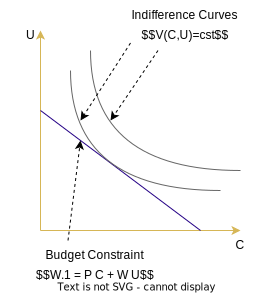
\includegraphics{assets/optimization.png}
\end{column}

\begin{column}{0.6\textwidth}
Un travailleur choisit de fournir du travail \(L\leq 1\).

Il peut soit :

\begin{itemize}
\tightlist
\item
  consommer un panier de biens \(C\) au niveau de prix \(P\)
\item
  profiter du temps libre \(U=1-L\)
\end{itemize}

Nous pouvons écrire la contrainte budgétaire : \[W 1 \geq P C + W U\]

L'utilité à maximiser
est\footnote{$\xi>0$ est l'élasticité de substitution entre la consommation et les loisirs.}\[V(C,u) = \log(C) + \xi U^{-\frac{1}{\xi}}\]
\end{column}
\end{columns}
\end{frame}

\begin{frame}{Offre de travail}
\phantomsection\label{offre-de-travail-1}
\framesubtitle{Résultat}

\begin{columns}[T]
\begin{column}{0.4\textwidth}
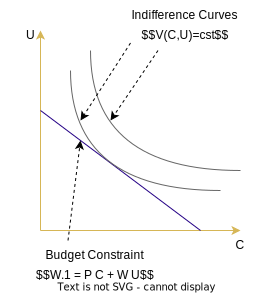
\includegraphics{assets/optimization.png}
\end{column}

\begin{column}{0.6\textwidth}
Le résultat de l'optimisation
donne\footnote{Les détails des calculs sont exposés dans l'exercice 3.}
:

\[\boxed{L^S = \left(\frac{W}{P}\right)^\xi}\]

L'offre de travail est une fonction croissante du salaire \emph{réel}.

\begin{itemize}
\tightlist
\item
  elle augmente lorsque les salaires augmentent
\item
  elle diminue lorsque le niveau des prix augmente
\end{itemize}

Le paramètre \(\xi\) est l'élasticité de l'offre de travail au salaire
réel
\end{column}
\end{columns}
\end{frame}

\begin{frame}{Coût du travail}
\phantomsection\label{couxfbt-du-travail}
La dernière relation peut être inversée pour obtenir le salaire que les
entreprises doivent proposer pour embaucher \(L\) travailleurs :

\[W(L) = P L^{\frac{1}{\xi}}\]

Nous voyons clairement que le salaire d'équilibre est :

\begin{itemize}
\tightlist
\item
  proportionnel au niveau des prix
\item
  croissant en fonction du nombre de travailleurs
\end{itemize}

Face à une demande plus élevée, toutes les entreprises pourront produire
davantage, mais feront face à des coûts croissants à mesure que les
travailleurs deviendront plus chers.
\end{frame}

\subsection{Le lien salaire-prix}\label{le-lien-salaire-prix}

\begin{frame}{Le lien salaire-prix}
Rappelons l'identité \(Y=L\), de sorte que \(W(L)=W(Y)\).

Résumons ce que nous avons jusqu'à présent :

\begin{itemize}
\tightlist
\item
  Marché des biens :

  \begin{itemize}
  \tightlist
  \item
    prix optimal : \(P^{\star} = (1+\mu) W(Y)\)
  \end{itemize}
\item
  Marché du travail

  \begin{itemize}
  \tightlist
  \item
    taux de salaire : \(W(Y) = P Y^{\xi}\)
  \end{itemize}
\end{itemize}

Comment ces deux marchés sont-ils liés? Quel type de dynamique
créent-ils?
\end{frame}

\subsection{L'équilibre naturel}\label{luxe9quilibre-naturel}

\begin{frame}{L'équilibre naturel}
\phantomsection\label{luxe9quilibre-naturel-1}
\textbf{Équilibre naturel} : niveau de production lorsque tous les prix
sont flexibles ou ont eu suffisamment de temps pour s'ajuster.

Ici, cela signifie que le prix \(P^{\star}\) fixé par les entreprises
doit être égal au niveau des prix \(P\)

Nous pouvons écrire : \[P = (1+\mu) \underbrace{P Y^{\xi}}_{W(Y)}\]

Ce qui donne : \[1=(1+\mu) Y^{\frac{1}{\xi}}\]

Cette équation détermine la production d'équilibre \(Y\). Notez
également que le niveau des prix a disparu. Il est indéterminé.
\end{frame}

\begin{frame}{Production naturelle}
\phantomsection\label{production-naturelle}
Le niveau de production naturelle est :
\[\boxed{Y^{nt}=\left(\frac{1}{1+\mu}\right)^{\xi}}\]

Remarques

\begin{itemize}
\tightlist
\item
  il diminue avec les majorations \(\mu\)
\item
  intuition : chaque entreprise est en monopole partiel et sa stratégie
  optimale consiste à rationner le marché pour augmenter les prix et les
  bénéfices
\end{itemize}
\end{frame}

\begin{frame}{Offre agrégée de long terme}
\phantomsection\label{offre-agruxe9guxe9e-de-long-terme}
\framesubtitle{Courbe LRAS}

\begin{columns}[T]
\begin{column}{0.48\textwidth}
\begin{figure}[H]

{\centering \includegraphics{assets/lras.png}

}

\caption{LRAS}

\end{figure}%
\end{column}

\begin{column}{0.48\textwidth}
\begin{itemize}
\tightlist
\item
  Production naturelle

  \begin{itemize}
  \tightlist
  \item
    ou l'offre avec des prix flexibles
  \item
    correspond à la vue classique
  \item
    est représentée comme une ligne verticale dans le plan \((\pi,y)\)
  \item
    est plus susceptible de se maintenir à long terme (les prix ont le
    temps de s'ajuster)
  \item
    est également appelée offre agrégée à long terme (LRAS)
  \end{itemize}
\item
  Lorsque les prix sont parfaitement flexibles, les politiques de
  demande sont inefficaces

  \begin{itemize}
  \tightlist
  \item
    elles n'augmentent que l'inflation
  \end{itemize}
\end{itemize}
\end{column}
\end{columns}
\end{frame}

\begin{frame}{offre agrégée à long terme}
\phantomsection\label{offre-agruxe9guxe9e-uxe0-long-terme}
\framesubtitle{Courbe LRAS}

\begin{columns}[T]
\begin{column}{0.48\textwidth}
\begin{figure}[H]

{\centering \includegraphics{assets/as.png}

}

\caption{LRAS}

\end{figure}%
\end{column}

\begin{column}{0.48\textwidth}
Entre les deux cas extrêmes :

\begin{itemize}
\tightlist
\item
  prix constants

  \begin{itemize}
  \tightlist
  \item
    aucune contrainte d'offre
  \item
    une façon de penser aux politiques de demande
  \end{itemize}
\item
  prix parfaitement flexibles

  \begin{itemize}
  \tightlist
  \item
    courbe verticale
  \item
    monde classique
  \end{itemize}
\end{itemize}

Pouvons-nous modéliser une situation où il y a un ajustement limité des
prix? Cela conduirait-il à une courbe des offres globales ascendante?

\begin{itemize}
\tightlist
\item
  c'est-à-dire une relation positive entre l'inflation et la production
  à court terme?
\end{itemize}
\end{column}
\end{columns}
\end{frame}

\section{Rigidités nominales}\label{rigidituxe9s-nominales}

\begin{frame}{Rigidités nominales}
\phantomsection\label{rigidituxe9s-nominales-1}
Pour nous éloigner de l'équilibre naturel, nous avons besoin de
certaines
\textbf{frictions}\footnote{Une friction est une force qui ralentit l'ajustement du marché en réponse à un écart temporaire par rapport à l'équilibre.}
soit dans le marché des biens, soit dans le marché du travail.

Explications les plus courantes :

\begin{itemize}
\tightlist
\item
  salaires rigides :

  \begin{itemize}
  \tightlist
  \item
    le marché du travail n'est pas en équilibre
  \end{itemize}
\item
  prix rigides :

  \begin{itemize}
  \tightlist
  \item
    les entreprises ne peuvent pas ajuster les prix librement
  \end{itemize}
\item
  mauvaise perception :

  \begin{itemize}
  \tightlist
  \item
    les entreprises ajustent les prix librement mais n'utilisent pas les
    bonnes informations
  \end{itemize}
\end{itemize}

Hypothèse centrale des nouveaux modèles keynésiens : certaines rigidités
\emph{nominales} ont des effets réels
\end{frame}

\subsection{Prix rigides}\label{prix-rigides}

\begin{frame}{Prix rigides}
\phantomsection\label{prix-rigides-1}
\framesubtitle{Les prix sont-ils réellement rigides?}

\begin{itemize}
\tightlist
\item
  Si les prix étaient flexibles, ils changeraient tout le temps

  \begin{itemize}
  \tightlist
  \item
    Les prix des actions sont mis à jour en continu (LSE : 126
    microsecondes)
  \end{itemize}
\item
  Il existe des statistiques sur les changements de prix : ils sont
  rigides (voir tableau ci-dessous)

  \begin{itemize}
  \tightlist
  \item
    Fréquence mensuelle des changements de prix : proportion des ajustés
    chaque mois
  \item
    Durée moyenne des prix : temps moyen nécessaire pour réviser un prix
  \end{itemize}
\end{itemize}

\begin{longtable}[]{@{}ccc@{}}
\toprule\noalign{}
& Zone euro (1996-2000) & États-Unis (1998-200) \\
\midrule\noalign{}
\endhead
Fréq mensuelle des changements de prix & 15,1\% & 21,5\% \\
Durée moyenne des prix & 13,0 mois & 9,6 mois \\
\bottomrule\noalign{}
\end{longtable}
\end{frame}

\begin{frame}{Quels prix sont les plus rigides?}
\phantomsection\label{quels-prix-sont-les-plus-rigides}
\begin{figure}[H]

{\centering \includegraphics[width=\textwidth,height=0.8\textheight]{assets/sectoral_spending.png}

}

\caption{Dépenses sectorielles et rigidité des prix}

\end{figure}%
\end{frame}

\begin{frame}{Prix rigides}
\phantomsection\label{prix-rigides-2}
\begin{itemize}
\item
  Nous modéliserons la situation où seulement une fraction
  \(\omega \in [0,1]\) des entreprises a la possibilité d'ajuster leurs
  prix à chaque période
\item
  Les biens sont vendus à deux prix différents :

  \begin{itemize}
  \tightlist
  \item
    \(P_{t-1}\) : ancien prix, toujours utilisé par les entreprises non
    ajustées
  \item
    \(P^{\star}_t\) : prix optimal fixé par les entreprises ajustées
  \end{itemize}
\item
  Ensuite, nous avons le prix d'un panier de consommation qui est une
  moyenne des deux
  prix\footnote{En général, dans la littérature, cette formule est une moyenne géométrique plutôt qu'une moyenne arithmétique. Cela est dû à la façon dont les paniers de consommation sont généralement définis et simplifie énormément les calculs.}

  \begin{itemize}
  \tightlist
  \item
    \(P_t = P_{t-1}^{(1-\omega)}(P^{\star})^{\omega}\)
  \end{itemize}
\end{itemize}
\end{frame}

\begin{frame}{Calculs}
\phantomsection\label{calculs}
Revenons à la décision de tarification optimale :
\[P^{\star}_t = (1+\mu) \overbrace{P_t Y_t^{\frac{1}{\xi}}}^{\text{Coût de la main-d'œuvre}}\]

Maintenant, à l'équilibre, les nouveaux prix fixés par les entreprises
optimisantes modifient le prix des paniers de consommation (et le
pouvoir d'achat des travailleurs), mais seulement partiellement :
\[P^{\star}_t = (1+\mu) {\underbrace{P_{t-1}^{(1-\omega)}(P^{\star}_t)^{\omega}}_{P_t}  Y^{\frac{1}{\xi}}}\]

Nous pouvons réécrire :
\[\left(\frac{P^{\star}_t}{P_{t-1}}\right)^{1-\omega} = (1+\mu) Y_t^{\frac{1}{\xi}} \Leftrightarrow Y_t = \left(\frac{1}{1+\mu}\right)^{\xi}\left(\frac{P^{\star}_t}{P_{t-1}}\right)^{\xi (1-\omega)}\]
\end{frame}

\begin{frame}{Production en équilibre}
\phantomsection\label{production-en-uxe9quilibre}
Le ratio \(\frac{P^{\star}_t}{P_{t-1}}\) est utile uniquement pour les
entreprises ajustantes, mais en réécrivant la formule de la moyenne des
prix comme
\(\frac{P^{\star}_t}{P_{t-1}}=\left(\frac{P_t}{P_{t-1}}\right)^{\frac{1}{\omega}}\),
nous obtenons une version plus agréable :

\[Y_t = \left(\frac{1}{1+\mu}\right)^{\xi}\left(\frac{P_t}{P_{t-1}} \right)^{\xi\frac{1-\omega}{\omega}}\]

Ou, en fonction de l'inflation :
\[\boxed{Y_t = \left(\frac{1}{1+\mu}\right)^{\xi}\left(1+\pi_t \right)^{
  \xi\frac{1-\omega}{\omega}}
}\]

Cette équation établit une relation positive entre l'inflation et la
production.
\end{frame}

\begin{frame}{Calculs}
\phantomsection\label{calculs-1}
Dans la dernière équation, nous reconnaissons la production naturelle :
\(Y_t^{nt} =\left( \frac{1}{1+\mu} \right)^{\xi}\)

\[Y_t = Y^{nt} \left(1+\pi_t \right)^{
  \xi\frac{1-\omega}{\omega}}
\]

Prenez les logarithmes pour obtenir une équation linéaire :
\[y_t - y^{nt}_t= \xi \frac{1-\omega}{\omega} \pi_t\]

Si nous posons \(\kappa = \frac{1}{\xi}\frac{\omega}{1-\omega}\), nous
obtenons notre version de la courbe de Phillips

\[\boxed{\kappa (y_t-y^{nt}_t) = \pi_t}\]
\end{frame}

\begin{frame}{Courbe de Phillips (William Phillips, 1958)}
\phantomsection\label{courbe-de-phillips-william-phillips-1958}
\begin{columns}[T]
\begin{column}{0.48\textwidth}
\includegraphics{assets/session_32.png}
\end{column}

\begin{column}{0.48\textwidth}
À l'origine, la courbe de Phillips était formulée comme une relation
négative entre l'inflation et le chômage.

~

Le chômage est évidemment lié au travail et le travail à la production -
dans notre modèle \(U=1-L=1-Y\)
\end{column}
\end{columns}
\end{frame}

\begin{frame}{Notre courbe de l'offre agégée}
\phantomsection\label{notre-courbe-de-loffre-aguxe9guxe9e}
\framesubtitle{Quelques commentaires}

Nous avons obtenu la courbe des offres globales comme :
\[\pi_t = \kappa (y_t- y^{nt}_t)\]

avec \[\kappa = \frac{1}{\xi} \frac{\omega}{1-\omega}\]

où \(\omega\) est la fraction d'entreprises.

Cette formulation englobe :

\begin{itemize}
\tightlist
\item
  l'offre agrégée à long terme : lorsque \(\omega=1\)
\item
  les prix rigides : lorsque \(\omega=0\)
\item
  tous les cas intermédiaires
\end{itemize}
\end{frame}

\begin{frame}{Notre courbe de l'offre agégée}
\phantomsection\label{notre-courbe-de-loffre-aguxe9guxe9e-1}
\framesubtitle{Quelques commentaires}

En cours de route, nous avons fait quelques simplifications par rapport
au cadre New Keynesian de référence :

\begin{itemize}
\tightlist
\item
  nous avons omis les chocs de productivité

  \begin{itemize}
  \tightlist
  \item
    nous les réintroduirons comme chocs dans \(y^{nt}_t\)
  \end{itemize}
\item
  nous n'avons incorporé aucune ``anticipation'' dans le comportement
  des entreprises. en principe, elles devraient

  \begin{itemize}
  \tightlist
  \item
    faire des prévisions de prix rationnelles pour fixer leurs prix
  \item
    maximiser leur profit intertemporel
  \end{itemize}
\item
  en fonction du choix de modélisation on on obtient des termes en:

  \begin{itemize}
  \tightlist
  \item
    \(\pi_{t-1}\) pour optimisation statique et extrapolation du trend
    (\(E_t \pi_{t+1}=\pi_t\)) \footnote<.->{c'est l'hypothèse retenue
      dans le poly.}
  \item
    \(\pi_{t+1}\) pour optimisation dynamique et anticipations
    rationnelle (modèle standard)
  \end{itemize}
\end{itemize}
\end{frame}

\begin{frame}{Prix rigides}
\phantomsection\label{prix-rigides-3}
\framesubtitle{Intuition de l'augmentation de la courbe des offres globales.}

Supposons que les prix partent du niveau d'équilibre à long terme

\begin{itemize}
\tightlist
\item
  Un choc crée une pression inflationniste (par exemple, la banque
  centrale baisse les taux d'intérêt)
\item
  Les prix devraient augmenter
\item
  Mais les entreprises ne peuvent pas ajuster facilement leurs prix
\item
  Au lieu d'augmenter leurs prix, elles produisent davantage
\item
  Et embauchent plus de travailleurs
\item
  La production est augmentée et le chômage est réduit
\end{itemize}

Nous avons vu dans les diapositives précédentes qu'il est possible de
donner un sens rigoureux à cette série d'événements.
\end{frame}

\subsection{Salaires rigides}\label{salaires-rigides}

\begin{frame}{Salaires rigides}
\phantomsection\label{salaires-rigides-1}
Il existe une théorie alternative qui génère également une courbe des
offres globales ascendante : la théorie des salaires rigides.

Si le marché du travail était sans friction, les salaires s'ajusteraient
immédiatement à la hausse et à la baisse.

Mais en pratique, tant les employeurs que les employés évitent les
baisses de salaire.

Il existe deux principales écoles de pensée pour expliquer pourquoi :

\begin{itemize}
\tightlist
\item
  les syndicats et la négociation salariale
\item
  la théorie du salaire d'efficience
\end{itemize}
\end{frame}

\begin{frame}{Les salaires sont-ils rigides?}
\phantomsection\label{les-salaires-sont-ils-rigides}
\begin{figure}[H]

{\centering \includegraphics[width=\textwidth,height=0.8\textheight]{assets/sticky_wages.png}

}

\caption{Répartition des changements de salaire non nuls, travailleurs
horaires, 1996 Panel}

\end{figure}%
\end{frame}

\begin{frame}{Salaires rigides}
\phantomsection\label{salaires-rigides-2}
\framesubtitle{Intuition de l'augmentation de la courbe des offres globales.}

Supposons que les salaires ne soient pas facilement renégociés à court
terme. Considérez la séquence d'événements suivante :

\begin{itemize}
\tightlist
\item
  Un choc crée une pression inflationniste (par exemple, la banque
  centrale imprime de l'argent)
\item
  Les prix ont tendance à augmenter
\item
  Comme les salaires réels chutent, les travailleurs demandent qu'ils
  soient réévalués
\item
  Mais les contrats ne sont pas facilement renégociés
\item
  Le coût des travailleurs reste bon marché
\item
  Les entreprises produisent davantage et augmentent l'emploi
\end{itemize}
\end{frame}

\subsection{Mauvaise perception}\label{mauvaise-perception}

\begin{frame}{Mauvaise perception}
\phantomsection\label{mauvaise-perception-1}
\framesubtitle{Îles Lucas}

\begin{figure}[H]

{\centering \includegraphics[width=0.3\textwidth,height=\textheight]{assets/lucas_islands.jpg}

}

\caption{Îles Lucas}

\end{figure}%

\begin{itemize}
\tightlist
\item
  B. Lucas a proposé une autre explication : les producteurs n'observent
  que les changements de prix des biens qu'ils
  vendent\footnote{Comme s'ils étaient chacun sur leur propre île comme dans l'histoire racontée par Lucas.},
  et ne savent pas si les changements observés sont idiosyncratiques ou
  liés à l'inflation globale. Ils perçoivent mal la nature de
  l'inflation.
\item
  Dans ce cadre, il a montré comment la production peut évoluer avec des
  chocs d'inflation \emph{inattendus}.
\end{itemize}
\end{frame}

\begin{frame}{Mauvaise perception}
\phantomsection\label{mauvaise-perception-2}
Supposons que les producteurs observent les prix de leur propre
industrie. Ils ne réalisent pas qu'ils sont indexés sur les prix
agrégés. Voici l'histoire :

\begin{itemize}
\tightlist
\item
  Un choc crée une pression inflationniste (par exemple, la banque
  centrale imprime de l'argent)
\item
  Les prix ont tendance à augmenter
\item
  Les producteurs d'une industrie donnée observent des prix plus élevés
  dans leur secteur
\item
  Ils croient (à tort) que leur industrie est relativement plus
  rentable\footnote{S'ils avaient su que tous les prix augmentaient, ils auraient su qu'ils ne sont pas plus rentables et n'auraient pas augmenté leur production.}
\item
  Ils décident de produire davantage et d'embaucher plus de travailleurs
\end{itemize}
\end{frame}

\begin{frame}{Mauvaise perception}
\phantomsection\label{mauvaise-perception-3}
\begin{figure}[H]

{\centering \includegraphics[width=\textwidth,height=0.6\textheight]{assets/inflation_dashboard.png}

}

\caption{Tableau de bord de l'inflation}

\end{figure}%

Avec une transparence accrue (consultez le
\href{https://www.ecb.europa.eu/stats/macroeconomic_and_sectoral/hicp/html/index.en.html}{tableau
de bord}) des banques centrales occidentales, ce canal est moins
pertinent de nos jours, sauf dans des conditions désordonnées.
\end{frame}

\section{Conclusion}\label{conclusion}

\begin{frame}{Guide d'apprentissage}
\phantomsection\label{guide-dapprentissage}
\framesubtitle{Pour comprendre}

\begin{itemize}
\tightlist
\item
  Comment les entreprises monopolistiques fixent-elles leurs prix ?
\item
  Qu'est-ce qui détermine le taux de salaire auquel les travailleurs
  sont prêts à travailler ?
\item
  Quelle est la production naturelle ?
\item
  L'intuition derrière les trois théories expliquant la courbe AS :

  \begin{itemize}
  \tightlist
  \item
    Prix rigides
  \item
    Salaires rigides
  \item
    Misperception
  \end{itemize}
\end{itemize}
\end{frame}

\begin{frame}{À venir}
\phantomsection\label{uxe0-venir}
\textbf{Fluctuations macroéconomiques} : Quels sont les chocs et comment
la banque centrale et le gouvernement peuvent-y répondre ?
\end{frame}



\end{document}
